\chapter{Available hardware - Chronos watch and tools}

\section{Hardware specification}

\begin{figure}[h!]
  \centering
  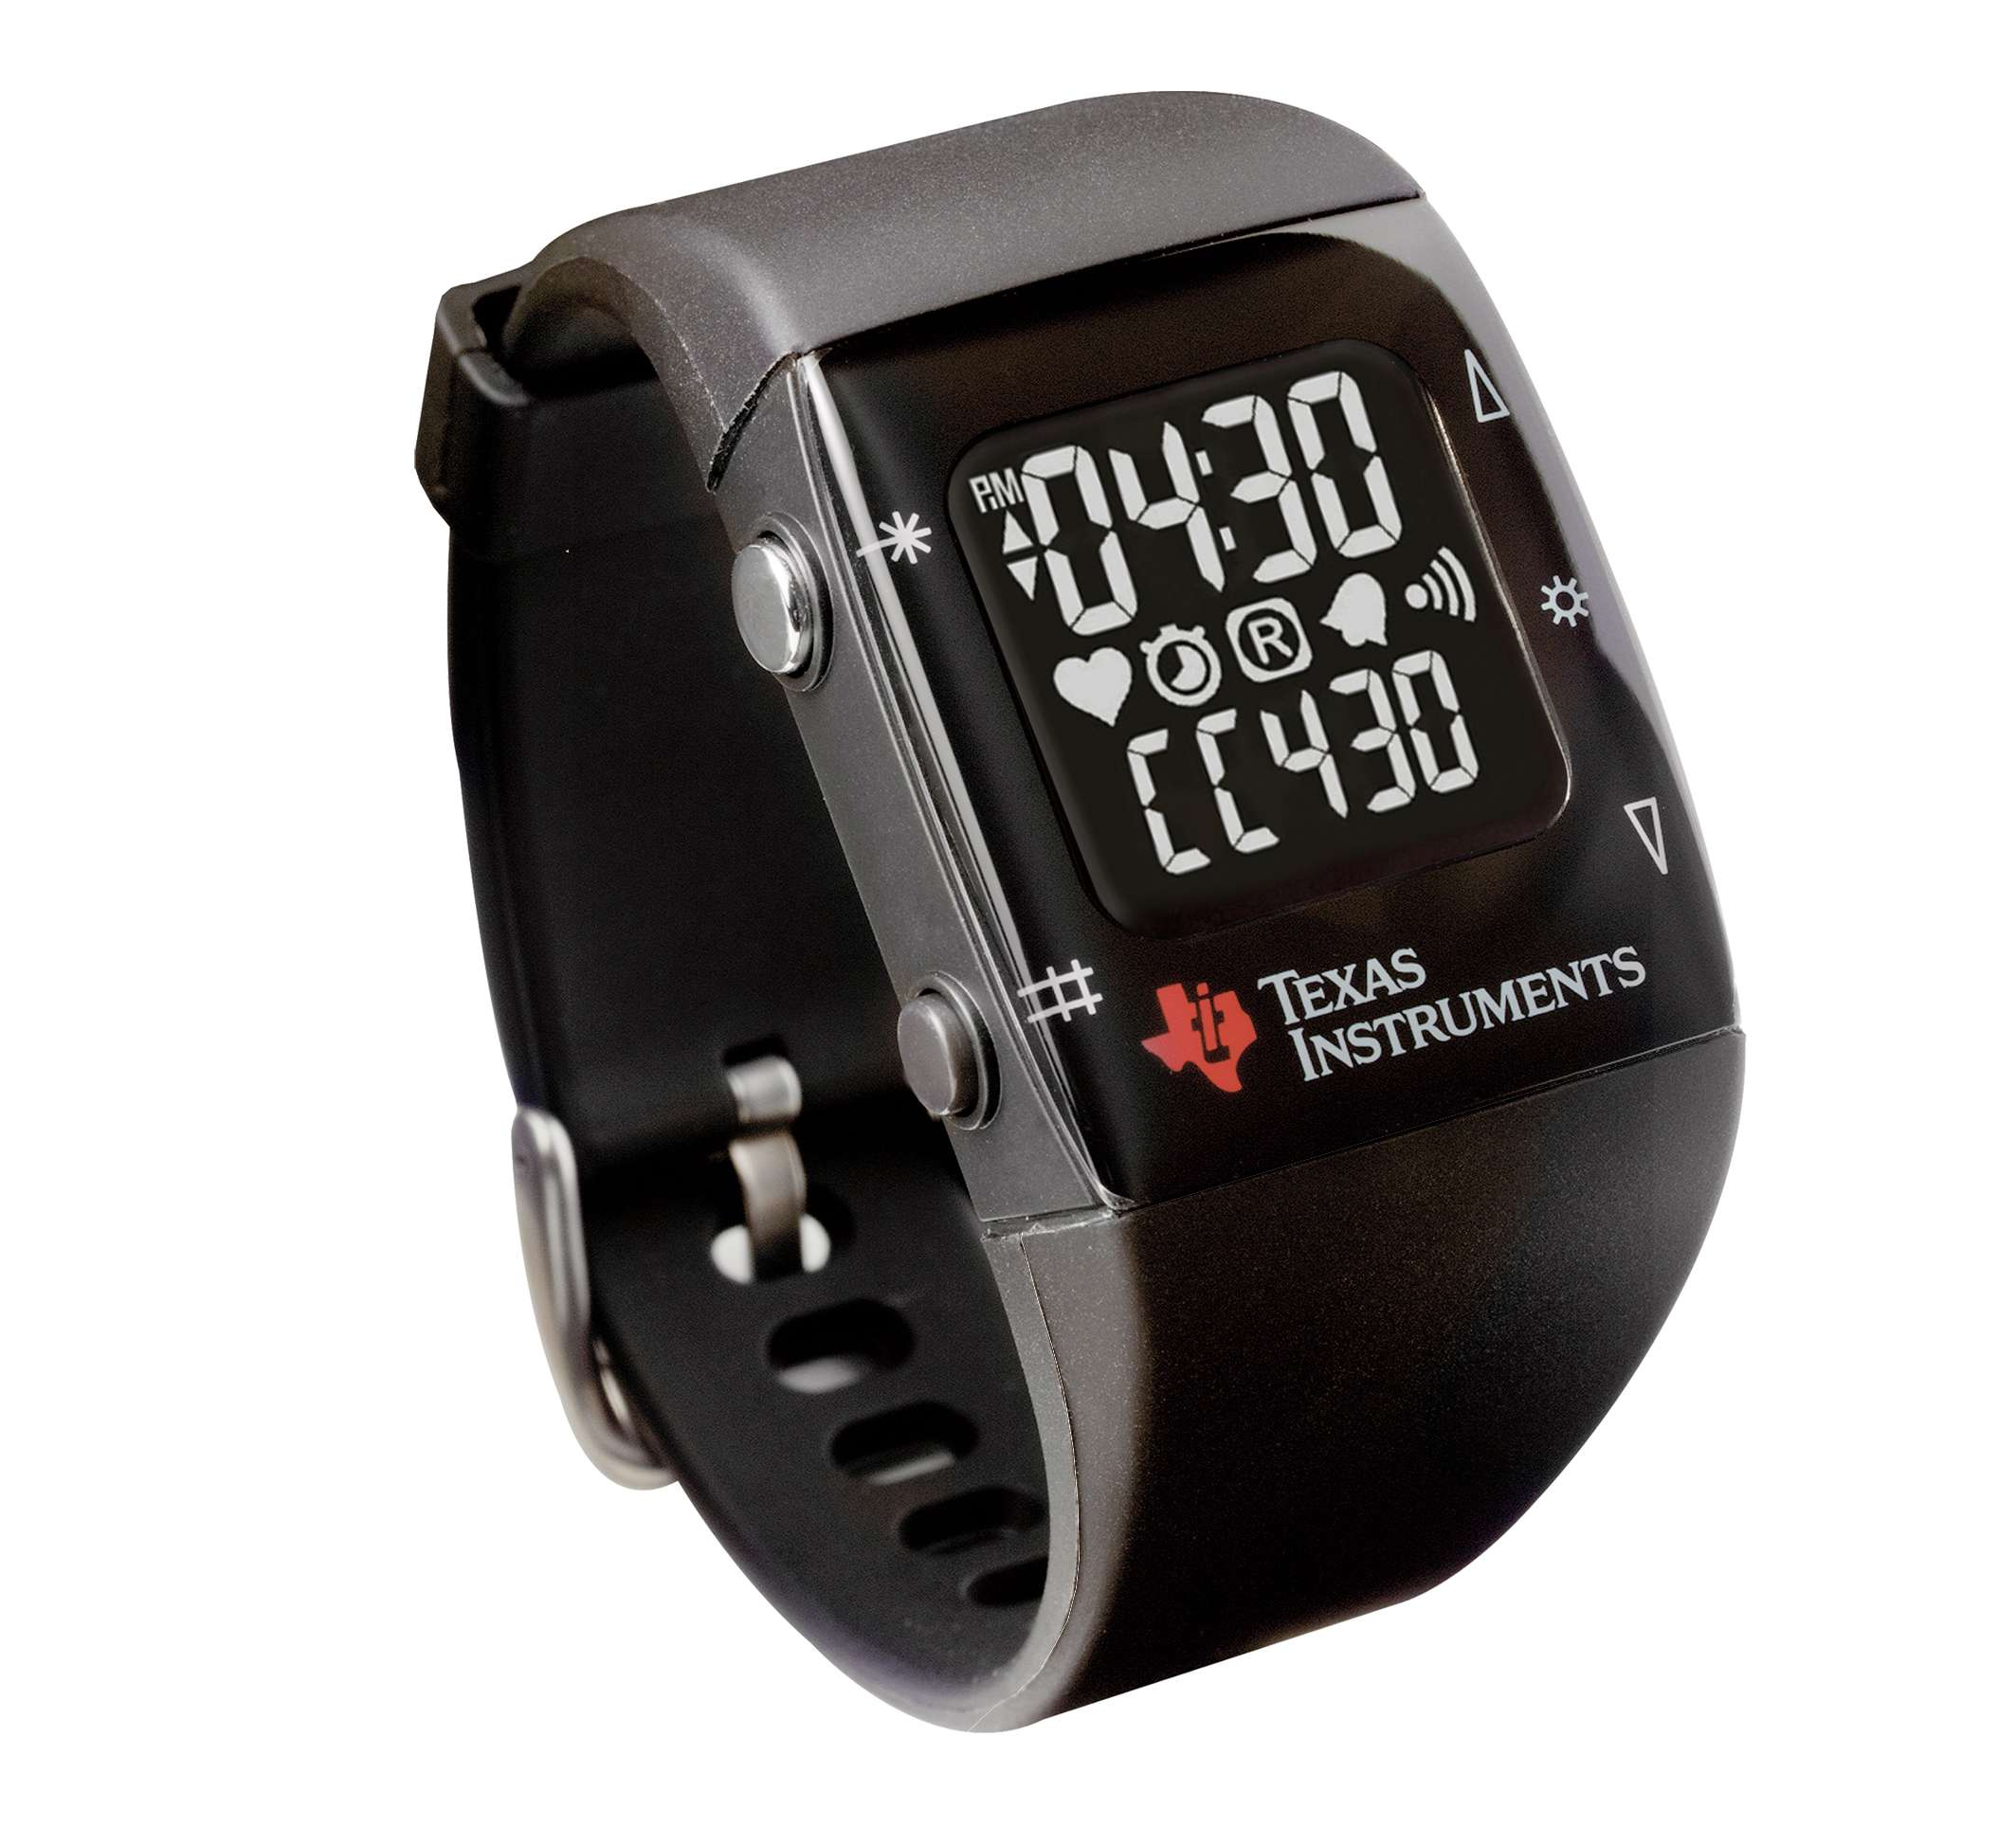
\includegraphics[width=0.9\textwidth]{img/chronos_watch.jpg}
  \caption{}
\end{figure}

\begin{commnet}
  Contents of this chapter
    # TI provides ez430-Chronos package with chronos watch (figure with watch box) and
      other tools
    # chapter will describe watch features, hinting applications they may be put to
      by the developer
    * Chronos watch
      # chronos shown on figure x is a battery powered hand watch. It's
        primary components are:
      * nine digit LCD screen, with button triggered back light all segments can
        be lit independently, allowing to form not only digits but also crude
        letters. All available segments and icons - figure. Blinking, and
        contrast control is also supported.
      * five user buttons
      * digital accelerometer
        <what can it detect - motion, free fall, ground, acceleration>
      * digital temperature and pressure sensor (altimeter?)
        <what can it be used to - elevation measuring>
      * programmable mcu - described in a separate section below
      * radio transceiver built in to the mcu - described in mcu section
    * Watch MCU (Mobile Compute Unit)
      # It has the low power MSP430 (Mixed Signal microProcessor) architecture.
        Belongs to the TI family of products code named CC430. Family datasheet
        describes most of chip functions.  The exact chip installed in the
        watch is code named CC430f6137. It's datasheet only describes details
        specific to this particular chip. What applications may be ran on the
        watch is limited by MCU's resources:
        * 32KB of flash memory. This is a non-volatile fast-read slow-write
          on-chip memory. It stores code and data. After reset MCU jumps to a
          location in this memory and starts executing instructions. I's amount
          may seem little but with modern code-size optimizing compilers quite
          complex applications are possible. For example this is just enough
          memory to fit a temperature monitoring application in which each node
          sends out it's readings and forwards ridings of other nodes in a way
          that enables results to reach a single sink node.
        * 4KB of RAM. It's operation consumes a lot of energy and this is the
          main limitation for it's amount. 4KB is however just enough to fit a
          temperature
          monitoring application mentioned above.
        * 20 Mhz of maximum clock speed. MSP430 RISC instructions are
          however much simpler than, for example x86 ones. To give a
          feel for this difference, 16 MHz (default in chronos) was
          compared to an Intel Core 2 x86 processor. .. <Floyd-Warshal
          comparison>
    * Additional hardware features of the MCU chip
      # There are certain functions that, though possible to implement in
        software are also easily implemented in hardware. Choosing the second
        approach saves both execution time and energy.  Also some features can
        only be implemented with hardware support.  Here we'll walk through most
        important ones available in the CC430f6137 MCU (and many other members of
        the CC430 family for that matter):
      * LPM support (Low Power Mode). The MCU can be in one of several
        so called power states. They are called Active, LPM0, LPM1.. 
        Each successive consumes less energy, by disabling various
        functions and peripherals. This mechanism is crucial for
        lengthening the battery life. To give the reader a better feel of
        how important that is, we list some crude battery life
        estimates^2(note on the assumptions) :
        * In Active mode (executing instructions) watch battery would
        last for a week (6.8 days)
        * If LPM0 or LPM1 was used this would grow to roughly 280 days
        * In LPM2 battery would last around 9 years
        * And finally in LPM3 or LPM4 if would last half a decade (52
        years)
        From this, it's clear that if the battery is to last years
        than MCU must spend most of the time in lowest power modes.
     * Timer_A allows to sets an alarm that will fire (interrupt) after specific
       period of time and execute certain piece of code. It's hard to
       imagine using low power modes without such functionality.
     * Real Time Clock - The RTC_A module provides a real-time clock
       and calendar function that can also be configured as a
       general-purpose counter. Chronos is a watch after all and needs
       calendar functions.
     * IO pins and interrupts - MCU has pins coming out of it's chip.
       Most of them can be configured as input, output or special
       function. In input they inform of the signal that's connected to
       them. In output mode they can generate high or low state^(short
       circuit warning). Special function mode connects the pin to an
       internal hardware component i.e. the LCD driver.
       Also it is possible to be notified (interrupt) if state of an
       input pin changes. This gives a good way to implement buttons.
     * CRC module - speeds up calculation of check sums. MSP430 MCUs
       are poor in doing certain types of operations like shifts and
       using this hardware leads to considerable speed improvements,
       especially on large data blocks.
     * AES128 Accelerator - Advanced Encryption Standard 128 is a very
       secure symmetric cipher. Implementing it's encryption and
       decryption algorithms (which are very complicated) in software
       would not only be very slow but would also waste a large
       amount of flash memory.
     * LCD_B hardware driver. There are many more LCD segments on the
       display than there are pins on the chip. This means that the
       chip must send more data than it's connection capacity. This is
       solved by spreading data over time. Chip selects a group of
       segments and lits only ones within this group. If groups are
       changed quickly enough human won't notice the blinking. However
       doing this in software would be very wasteful. LCD_B hardware
       driver does this instead.
     * Universal Serial Communication Interface (USCI) is a special
       hardware driver that can be configured to pose as one of
       standard communication interfaces. Most notably these are SPI
       (Serial Peripheral Interface), I^2C (Inter-Integrated Circuit)
       and UART (Universal Asynchronous Receiver/Transmitter). Though
       cumbersome, each one can be implemented in software, however
       hardware support increases performance by an order of
       magnitude.
     * Port remapping. Typically special functions are hard-connected to
       certain chip pins. I.e. UART's Tx and Rx may be mapped to pins
       P1.0 and P1.1. If we had two components that wanted to
       communicate with the MCU chip via UART, some external circuitry
       would be needed to reconnect the pins on demand. This isn't
       however necessary in CC430 family, because such functionality is
       built-in and known as port remapping. Special functions can
       be reconnected to arbitrary IO pins during MCU operation.
     * RF1A module is 868MHz radio transceiver, which is capable of
     sending and receiving short packets of data (around 50 bytes in
     length). Typically such modules are implemented in separate
     chips. CC430 family however has has it built in, which decreases
     production costs. Also radio module is very power consuming and
     must be used sparingly.
     * REF is a reference voltage generator. Some components like the
     LCD require a certain electric voltage for their operation.
     Others perform comparisons of external voltages to the reference
     voltage. It is very convenient to generate such voltage without
     help of external circuitry.
     * Comp_B is a voltage comparator. It is a circuit that can
     compare two voltages and tell which one is higher. Also one of
     them could be a reference voltage of known value. Comparators are
     used to interface real world signals to digital circuitry
     * ADC12_A is an analog to digital converter module. Conceptually
     it's a generalised comparator ^(footnote, about realisation),
     because it returns multiple bits of information instead of one.
     An ADC circuit can very quickly measure the value of some
     external voltage. Thus if you wanted to construct a thermometer
     you would connect a thermo-resistor (resistance of which reflects
     it's temperature) to the reference voltage and measure the
     resulting voltage with ADC. From that result temperature can be
     derived.


\end{comment}

% Vim settings:
% vim: set textwidth=70:
% vim: set formatoptions+=t:
